\chapter{Graph Coloring}

\begin{definizione}[$\alpha$-coloring]
    Sia $G = (V, E)$ un grafo. Un $\alpha$-\textit{coloring} di $G$ è un'etichettamento dei vertici di $G$ tale che nessun coppia di vertici adiacenti condivida la stessa etichetta. Formalemnte, è una funzione
    \[
        c: V \to \{1, 2, \ldots, \alpha\}
    \]
    è un $\alpha$-coloring se per ogni $(u, v) \in E$, $c(u) \neq c(v)$.
\end{definizione}

Nel mondo centralizzato, questo è un problema NP-completo, ma in un contesto distribuito, possiamo trovare soluzioni efficienti con algoritmi che sfruttano la comunicazione tra i nodi.

\section{Deterministic Distributed Graph Coloring}

Ci troviamo in un contesto $\mathcal{LOCAL}$, ossia ad ogni nodo è assegnata un'etichetta univoca $id(v)$ che solo lui conosce, ogni nodo può comunicare solo con i suoi vicini in \textbf{round discreti e sincroni}. Ogni nodo può eseguire un numero di computazioni potenzialmente illimitato e può inviare messaggi distinti a ciascuno dei suoi vicini in ogni round, e tali messaggi arrivano entro la fine del round.

Consideriamo ora il problema del \textbf{coloring} restringendolo a grafi $\Delta$-regolari, ossia grafi in cui ogni nodo ha al più $\Delta$ vicini. L'obiettivo è trovare un $(\Delta + 1)$-coloring in modo distribuito, poiché è noto che $\Delta + 1$ colori sono sufficienti per colorare qualsiasi grafo con grado massimo $\Delta$. In particolare:

\begin{itemize}
    \item $P_{init}$: una configurazione iniziale che consiste in un $\alpha$-coloring con $\alpha > \Delta + 1$.
    $$C_{init}: V \to [1, \alpha], \quad \forall v \in V, \; C_{init}(v) \in [1, \alpha]$$
    \item $P_{final}$: una configurazione finale che consiste in un $(\Delta + 1)$-coloring.
    $$C_{final}: V \to [1, \Delta + 1], \quad \forall v \in V, \; C_{final}(v) \in [1, \Delta + 1]$$
    \item Restrizioni standard più modello $\mathcal{LOCAL}$: $R = R \cup \mathcal{LOCAL}$.
\end{itemize}

\subsection{Basic Color Reduction Procedure - BCP}

La \textbf{BCP} è una tecnica deterministica che permette di ridurre il numero di colori in $G$ da $\alpha$ a $\Delta + 1$ in $O(\alpha - (\Delta + 1))$ rounds. 

Ogni nodo $v$ esegue in parallelo i seguenti passi per ogni round:

\begin{enumerate}
    \item Trasmette il proprio colore $c(v)$ a tutti i vicini $u \in N(v)$ e riceve il colore $c(u)$ da ciascuno di essi.
    \item Seleziona un nuovo colore $c'(v)$ dall'insieme dei colori \emph{disponibili}, definito come:
    \[
        \mathcal{A}(v) = \{1, \dots, k\} \setminus \{c(u) \mid u \in N(v)\}
    \]
    \item Se $c'(v) \neq c(v)$, aggiorna il proprio colore: $c(v) \leftarrow c'(v)$.
\end{enumerate}

Il processo termina quando ogni nodo $v$ ha un colore distinto da quello di tutti i suoi vicini, ovvero quando la colorazione è \emph{propria}.

\begin{algorithm}
\caption{BCP}
\begin{algorithmic}[1]
\For{node $v \in V$}
    \For{phase $k = \alpha, \alpha-1, \dots, \Delta+2$}
        \State \textbf{send} $C(v)$ to $N(v)$
        \State \textbf{receive} $C(u)$ for all $u \in N(v)$
        \If{$C(v) = k$}
            \State choose $j \in \{1, \dots, k-1\} \setminus C(N(v))$
            \State $C(v) \leftarrow j$
        \EndIf
    \EndFor
\EndFor
\end{algorithmic}
\end{algorithm}

\begin{teorema}[Correttezza]
    Il protocollo BCP ritorna un $(\Delta + 1)$-coloring
    \[
        C_{final}: V \to [1, \Delta + 1]
    \]
    \begin{proof}
        Valgono i seguenti fatti:
        \begin{description}
            \item[FACT 1:] Poiché $k > \Delta + 1$ e poichè ad ogni round $k$, il nodo $v \in V:\ c(v) = k$ ha al più $\Delta$ vicini che possono avere $\Delta$ colori distinti, allora il nodo $v$ ha almeno un colore disponibile $j < k:\ j \in [1, k-1] \setminus C(N(v))$.
            
            Formalmente, poiché $|N(v)| \leq \Delta$ e $k > \Delta + 1$, abbiamo:
            \[
                |[k-1] \setminus C(N(v))| = |[k-1]| - |C(N(v))| > \Delta - \Delta = 0 \quad (\geq 1)
            \]
            Quindi, esiste almeno un colore $j$ che non è utilizzato dai vicini di $v$.
            \item[FACT 2:] Al termine di ogni round $k > \Delta + 1$, la colorazione $C_k: V \to [1, k-1]$ è legale. Poiché si parte da una colorazione legale, e ad ogni round solo i nodi con colore $k$ cambiano il loro colore (che per definizione di colorazione legale, non sono vicini), e ogni nodo $v$ che cambia colore sceglie un nuovo colore $j$ che è disponibile (non utilizzato dai vicini), allora la colorazione rimane legale.
        \end{description}
    \end{proof}
\end{teorema}

\begin{teorema}[Time Complexity \& Message Complexity]
    Vale il seguente:
    \begin{itemize}
        \item $T[BCP] = O(\alpha - (\Delta + 1))$. Se $\alpha \in O(n)$, allora $T[BCP] = O(n - \Delta)$. Inoltre, il caso peggiore si verifica quando $\Delta = O(1)$.
        \item $M[BCP] = O(m \cdot (\alpha - \Delta))$ oppure se $\alpha \in O(n)$, allora $M[BCP] = O(m \cdot (n - \Delta))$.
    \end{itemize}
\end{teorema}

\subsection{Khun-Wattenhofen Procedure}

Vediamo ora una procedura che permette di velocizzare la riduzione dei colori da $\alpha > 2(\Delta + 1)$ a $\Delta + 1$ in tempo $O(\Delta \log\frac{\alpha}{\Delta})$ invece che $O(\alpha - (\Delta + 1))$.

L'idea è di eseguire BCP in modo parallelo, di seguito i passi:

\begin{enumerate}
    \item Partizionare l'insieme dei nodi $V$ in $k = \left\lceil \frac{\alpha}{\Delta + 1} \right\rceil$ sottoinsiemi disgiunti $V_1, V_2, \dots, V_k$ tali che
    \[
        V_i = \{v \in V \mid C(v) \in [(i-1)(\Delta + 1) + 1, i(\Delta + 1)]\}
    \]
    \item Eseguire BCP in parallelo sul grafo indotto $G_{i, (i + 1)} = (V_i \cup V_{i+1}, E)$.
    Qui si distinguono due casi:
    \begin{itemize}
        \item   Se $k$ è pari, allora eseguiamo BCP in parallelo sui grafi indotti $G_{i, i+1}$ per $i = 1, 3, \dots, k-1$, dove la colorazione indotta da $C_{init}$ è 
        \[
            F_{i, i+1}: V_i \cup V_{i+1} \to [(i-1)(\Delta + 1) + 1, (i + 1)(\Delta + 1)]
        \]
        \item   Se $k$ è dispari, allora eseguiamo BCP in parallelo sui grafi indotti $G_{i, i+1}$ per $i = 1, 3, \dots, k-4$ e su $G_{k-2, k-1, k}$, dove la colorazione indotta da $C_{init}$ è
        \[
            F_{i, i+1}: V_i \cup V_{i+1} \to [(i-1)(\Delta + 1) + 1, (i + 1)(\Delta + 1)]
        \]
         e
        \[
            F_{k-2, k-1, k}: V_{k-2} \cup V_{k-1} \cup V_k \to [(k-3)(\Delta + 1) + 1, \alpha]
        \]
    \end{itemize}
    
    imponendo il numero di rounds $k = i(\Delta + 1) \dots (i+1)(\Delta + 1)$. 
    
    Questo grafo ammette una colorazione con al più $2(\Delta + 1)$ colori, quindi BCP può essere eseguito in $O(\Delta)$ rounds per ridurre i colori a $\Delta + 1$.
    \item Ripetere il passo 1 e 2 fino a quando il numero di colori è ridotto a $\Delta + 1$.
\end{enumerate}

\textbf{Esempio}

Consideriamo un grafo con $\Delta = 2$ e $\alpha = 11$. In questo caso, $k = \lceil \frac{11}{3} \rceil = 4$, quindi partizioniamo i nodi in quattro sottoinsiemi $V_1, V_2, V_3, V_4$ come nella figura \autoref{fig:khunProcedure}. Successivamente, eseguiamo BCP in parallelo sui grafi indotti $G_{12}. G_{34}$.

Consideriamo $\texttt{BCP}(G_{12})$. Allora le fasi vanno da $k = 3, \dots, 6$. L'\texttt{if c(v) == k} verrà eseguito sarà per $c(v) \in {3, 5, 6}$.
\begin{itemize}
    \item Se $c(v) = 3$, allora $v$ sceglierà un nuovo colore $j \in \{1, 2\} \setminus \{2\} = \{1\}$.
    \item Se $c(v) = 5$, allora $v$ sceglierà un nuovo colore $j \in \{1, 2, 3, 4\} \setminus \{6\} = \{1, 2, 3, 4\}$.
    \item Se $c(v) = 6$, allora $v$ sceglierà un nuovo colore $j \in \{1, 2, 3, 4, 5\} \setminus \{5\} = \{1, 2, 3, 4\}$.
\end{itemize}

In questo modo, come possiamo osservare, il numero di colori viene ridotto almeno di uno ad ogni round.

\begin{figure}[h]
    \centering
    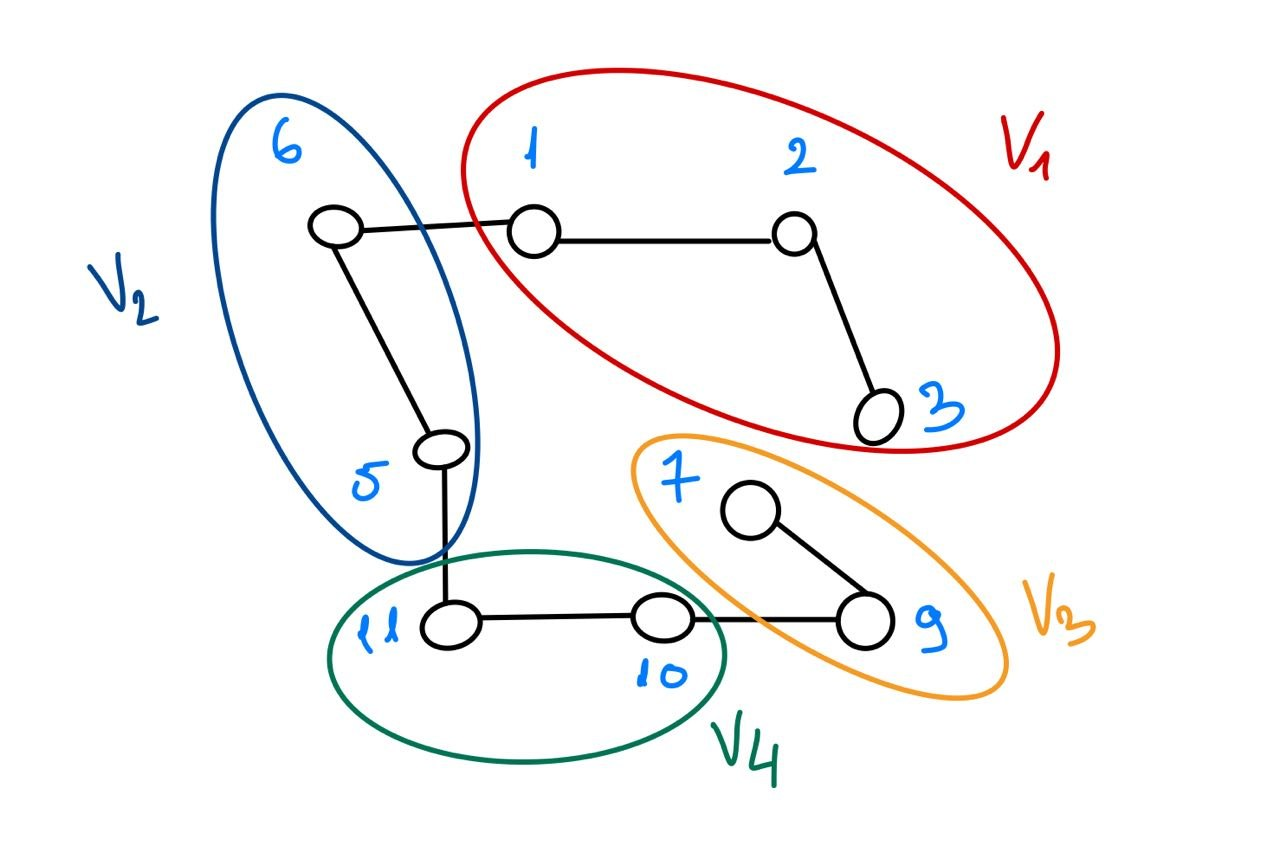
\includegraphics[width=0.4\textwidth]{images/khunProcedure.jpg}
    \caption{Esempio di partizione del grafo.}
\end{figure}\label{fig:khunProcedure}

Dopo un'iterazione di questa procudera parallela, il numero di colori sarà ridotto a $\alpha' = \lceil \frac{\alpha}{2} \rceil$. Cosi facendo, in tempo $O(\Delta)$ abbiamo \textbf{dimezzato} i colori della colorazione iniziale. Ripetendo, ogni $O(\Delta)$ si dimezza il numero di sottoinsiemi, e dopo $\log(\frac{\alpha}{\Delta})$ iterazioni avremo ridotto il numero di colori a $\Delta + 1$. In totale, la complessità temporale è $O(\Delta \log\frac{\alpha}{\Delta})$.

\section{Randomized Distributed Graph Coloring}

Un approccio probabilistico molto usato per risolvere questa tipologia di problemi distribuiti (non solo il \texttt{Graph Coloring}, ma per esempio anche il \texttt{Maximal Independent Set}) è il seguente: il protocollo procede per \textbf{fasi}, dove in ciascuna di esse ogni nodo sceglie casualmente un valore da un insieme appropriato di colori. In base al colore scelto, e a quello scelto dai propri vicini, ogni nodo deve prendere la decisione finale di adottare il colore scelto e terminare il protocollo, oppure di continuare alla fase successiva.

Osservare che tutti i nodi che prendono una decisione finale formano un sottoinsieme della soluzione finale. Perciò basta rimuovere i nodi che hanno terminato il protocollo, e procedere alla stessa maniera però sul grafo residuo. Un requisito importante che una soluzione parziale deve necessariamente avere è che essa non solo deve essere corretta nel relativo sottoinsieme di vertici, ma anche rispetto all'unione di tutti i sottoinsiemi rimossi nelle fasi successive. Il protocollo termina quando verranno rimossi tutti i nodi dal grafo, ovvero quando tutti i nodi avranno scelto definitivamente il proprio colore.

\subsection{Rand-2$\Delta$}

Definiamo formalemente il problema del \texttt{Rand-$2\Delta$-Coloring}:
\begin{itemize}
    \item $P_{init}$: Una colorazione iniziale dei nodi $C_{init}: V \to [\alpha]$ con $\alpha > 2\Delta$.
    \item $P_{final}$: Una colorazione finale dei nodi $C_{final}: V \to [2\Delta]$.
    \item Restrizioni standard più modello $\mathcal{LOCAL}$: $R = R \cup \mathcal{LOCAL}$.
\end{itemize}

Entriamo ora nel merito del protocollo \texttt{Rand-$2\Delta$} che calcola in maniera distribuita una $2\Delta$ colorazione di un grafo $G$ in accordo all'approccio precedente, dove $\Delta$ è il grado massimo di $G$. Ad ogni fase, ogni nodo $v$ campiona \textit{u.a.r.} un colore $c(v)$ dall'insieme $[2\Delta]=\{1,2,\ldots,2\Delta\}$. Indichiamo con $F_v$ l'insieme dei colori scelti definitivamente dai vicini di $v$, e con $T_v$ l'insieme dei colori scelti (temporaneamente) dai vicini di $v$ nel corrente round. Se $c(v) \notin F_v \cup T_v$, allora $c(v)$ diventa il colore definitivo di $v$, e in tal caso il nodo termina il protocollo. Altrimenti $v$ scarta $c(v)$ e continua alla fase successiva.

\begin{algorithm}
\caption{Procedure \textsc{Rand-2Delta}($G$)}
\begin{algorithmic}[1]

\State An algorithm for each vertex $v \in V$.
\State Initially $T_v = \emptyset$, $F_v = \emptyset$, for each $v \in V$.
\State \textit{$T_v$ is the set of temporary colors selected by neighbors of $v$.}
\State \textit{$F_v$ is the set of final colors selected by neighbors of $v$.}

\For{each round}
    \State $T_v = \emptyset$
    \State $c(v) :=$ draw a color from $[2\Delta]$ u.a.r., independently of other vertices
    \State $\texttt{send}(c(v)) \to N(v)$
    \For{each received color $c(u)$ from a neighbor $u$}
        \State $T_v := T_v \cup \{c(u)\}$
    \EndFor
    \If{$c(v) \notin T_v \cup F_v$}
        \State $\texttt{send}(\texttt{final} \; c(v)) \to N(v)$
        \State select $c(v)$ as the final color $\varphi_v$ of $v$ and \textbf{terminate}
    \Else
        \For{each received message $\texttt{final} \; c(u)$ from a neighbor $u$}
            \State $F_v := F_v \cup \{c(u)\}$
        \EndFor
        \State discard $c(v)$ and continue to the next round
    \EndIf
\EndFor

\end{algorithmic}
\end{algorithm}

\newpage

\begin{teorema}[Correttezza]
    Se tutti i nodi terminano, allora il protocollo \texttt{Rand-$2\Delta$} calcola una $2\Delta$-colorazione del grafo $G$ in input.
    \begin{proof}
        Sappiamo con certezza che la colorazione finale $\varphi$ è una $2\Delta$-colorazione di $G$, perché per costruzione tutti i colori scelti dai nodi sono nell'insieme $[2\Delta]$, perciò serve solamente dimostrare che la colorazione $\varphi$ sia legale.

        Consideriamo due nodi adiacenti $u$ e $v$, e supponiamo per assurdo che alla fine del protocollo, $\varphi(u) = \varphi(v)$. Certamente i due nodi non possono aver terminato il protocollo nello stesso round, in quanto sarebbe accaduto che $c(u) \in T_u$ e $c(v) \in T_v$ (il controllo qui dentro non sarebbe false, vedi \texttt{riga 12}). Allora siano $i$ e $j$ i rounf in cui i nodi $u$ e $v$ hanno terminato ed assumiamo senza perdita di generalità che $i < j$. Allora dal round $i$ in poi, il colore definitivo $\varphi(u)$ sarà presente in $F_v$. Perciò, per costruzione dell'algoritmo, il colore definitivo $\varphi(v)$ sarà scelto al tempo $j$ in modo tale che $\varphi(v) \notin F_v$ (la condizione a \texttt{riga 12} sarà true), e quindi $\varphi(v) \neq \varphi(u)$, il che è una contraddizione.
    \end{proof}
\end{teorema}

\begin{teorema}[Time Complexity]
    Durante l'esecuzione del protocollo \texttt{Rand-$2\Delta$} tutti i nodi terminano la loro esecuzione entro $O(\log n)$ rounds con alta probabilità, $1 - \frac{1}{n^c}$ per una costante $c > 0$.
    \begin{proof}
        Consideriamo un qualisiasi nodo $v \in V$ e calcoliamo la probabilità che $v$ termini nel round $i$ condizionato al fatto che non ha terminato prima, per ogni $i \geq 1$.
        
        Osserviamo che $|T_v \Cup F_v| \leq \Delta$ perché ogni vicino di $v$ contribuisce con al più un colore a questo insieme, e inoltre $|N(v)| \leq \Delta$. Di conseguenza $v$ ha a disposizione \textbf{almeno} $\Delta$ colori valori per la colorazione finale nell'insieme $[2\Delta] \setminus (T_v \cup F_v)$. Perciò la probabilità che $v$ scelga un colore valido finale sarà almeno
        \[
            P(c(v) \notin T_v \cup F_v) = \frac{|[2\Delta] \setminus (T_v \cup F_v)|}{|[2\Delta]|} \geq \frac{\Delta}{2\Delta} = \frac{1}{2}
        \]

        Quindi, assumento che $v$ non termina \textbf{prima} del round $i$, la probabilità che termini al round $i$ è almeno $\frac{1}{2}$ \textbf{indipendentemente} dagli altri nodi.
        \[
            P(v \text{ termina al tempo } i \mid v \text{ non termina prima di } i) \geq \frac{1}{2}
        \]

        Viceversa, la probabilità che un dato nodo $v$ \textbf{non} termina entro il passo $i$ sarà al più $2^{-i}$. Facendo \textit{union bound} possiamo calcolare la probabilità che esista un nodo $v$ che entro il tempo $i$ non ha ancora finito come segue:
        \[
            P(\exists v \in V: v \text{ non termina entro } i) \leq \sum_{v \in V} P(v \text{ non termina entro }i) \leq n \cdot 2^{-i}
        \]

        Per $i = c \log n$ con $c > 0$, otteniamo che la probabilità che esista un nodo $v$ che non ha terminato entro il tempo $i$ è al più $\frac{1}{n^c}$, e di conseguenza la probabilità che tutti i nodi terminino entro il tempo $i$ è almeno $1 - \frac{1}{n^c}$. Quindi, con alta probabilità, tutti i nodi terminano entro $O(\log n)$ rounds.
    \end{proof}
\end{teorema}

\subsection{Rand-$\Delta$+}

Il protocollo \texttt{Rand-$\Delta$+} è una variante del protocollo \texttt{Rand-$2\Delta$} che permette di ridurre il numero di colori finali da $2\Delta$ a $\Delta + 1$. 

L'idea è quella che ogni nodo ad ogni iterazione deve prima partecipare ad una lotteria, e solo se vince la lotteria, allora può campionare un colore da $[\Delta + 1]$ e tentare di terminare. Nello specifico, le modifiche effettuate al protocollo iniziale sono le seguenti:
\begin{itemize}
    \item Ogni nodo $v \in V$ che partecipa alla fase $i$ sceglie \textit{u.a.r.} un bit $c(v) \in \{0,1\}$; se $c(v) = 0$, allora $v$ non partecipa alla scelta di un colore e viene direttamente fatto passare alla fase successiva.
    \item Ogni nodo $v \in V$ che partecipa alla fase $i$ (ossia quelli che hanno scelto $c(v) = 1$) sceglie \textit{u.a.r.} un colore $col(v)$ dalla palette $[\Delta + 1] \setminus F_v$. A questo punto il protocollo esegue come \texttt{Rand-$2\Delta$}.
\end{itemize}

\begin{teorema}[Correttezza]
    Se tutti i nodi terminano, allora il protocollo \texttt{Rand-$\Delta$+} calcola una $(\Delta + 1)$-colorazione del grafo $G$ in input.
\end{teorema}

\begin{teorema}[Time Complexity]
    Durante l'esecuzione del protocollo \texttt{Rand-$\Delta$+} tutti i nodi terminano la loro esecuzione entro $O(\log n)$ rounds con alta probabilità, $1 - \frac{1}{n^c}$ per una costante $c > 0$.
\end{teorema}
